% Figure 4 -- the two pipelines, drawn once in TikZ.
%
%   TRANSLATION          what happens once, off the board
%   INFERENCE -- XAVIER  what happens every frame, on the board
%
% Build:  bash analysis/build_latex.sh fig04_pipeline
%
% Six boxes per section and one arrow between them. Square corners, hairline
% rules, one accent colour per model stage and nothing else: at print size the
% reader should get the order of the stages and the handoff between the two
% sections without reading a single caption.
\documentclass[border=3pt]{standalone}
\usepackage[T1]{fontenc}
\usepackage{mathptmx}                     % Times, as the conference templates use
\usepackage{tikz}
\usetikzlibrary{arrows.meta,positioning,calc}

\definecolor{ink}{HTML}{15191C}
\definecolor{muted}{HTML}{6B7780}
\definecolor{rule}{HTML}{B9C2C9}
\definecolor{vision}{HTML}{0B6B63}
\definecolor{prefill}{HTML}{1D3F6B}
\definecolor{decode}{HTML}{8A3F08}
\definecolor{expert}{HTML}{473C6B}
\definecolor{store}{HTML}{55606B}

\tikzset{
  blk/.style={
    draw=black, line width=0.5pt, fill=white,
    inner xsep=2pt, inner ysep=3.5pt, minimum height=9mm, text width=17mm,
    align=center, font=\scriptsize, text=ink},
  acc/.style={draw=#1, line width=0.9pt, text=#1},
  kvbox/.style={
    draw=black, line width=0.6pt, fill=white, inner sep=3pt,
    align=center, font=\scriptsize, text=store},
  fl/.style={-{Stealth[length=3.4pt,width=2.6pt]}, draw=black, line width=0.5pt},
  bi/.style={{Stealth[length=3.4pt,width=2.6pt]}-{Stealth[length=3.4pt,width=2.6pt]},
             draw=black, line width=0.5pt},
  hand/.style={-{Stealth[length=4pt,width=3pt]}, draw=black, line width=0.6pt,
               densely dashed},
  lbl/.style={font=\tiny, text=muted, inner sep=1.5pt},
  ttl/.style={font=\scriptsize\bfseries, text=black, inner sep=0pt},
}
\newcommand{\two}[2]{#1\\[-1.5pt]{\tiny\color{muted}#2}}

\begin{document}
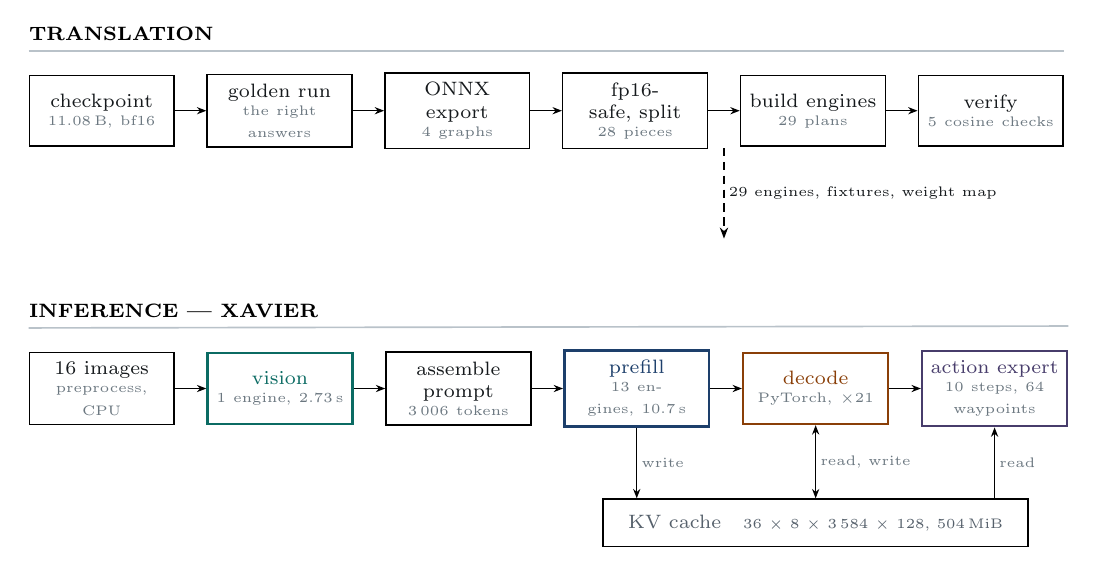
\begin{tikzpicture}[node distance=4mm]

% =====================================================================
\node[blk] (ckpt) {\two{checkpoint}{11.08\,B, bf16}};
\node[blk, right=of ckpt]  (gold)  {\two{golden run}{the right answers}};
\node[blk, right=of gold]  (exp)   {\two{ONNX export}{4 graphs}};
\node[blk, right=of exp]   (cut)   {\two{fp16-safe, split}{28 pieces}};
\node[blk, right=of cut]   (build) {\two{build engines}{29 plans}};
\node[blk, right=of build] (ver)   {\two{verify}{5 cosine checks}};

\foreach \a/\b in {ckpt/gold, gold/exp, exp/cut, cut/build, build/ver}
  \draw[fl] (\a) -- (\b);

\draw[rule, line width=0.6pt]
  ($(ckpt.north west)+(0,3mm)$) -- ($(ver.north east)+(0,3mm)$);
\node[ttl, anchor=south west] at ($(ckpt.north west)+(0,4.2mm)$) {TRANSLATION};

% =====================================================================
\coordinate (base) at ($(ckpt.south west)+(0,-26mm)$);
\node[blk, anchor=north west] (img) at (base) {\two{16 images}{preprocess, CPU}};
\node[blk, acc=vision,  right=of img] (vis) {\two{vision}{1 engine, 2.73\,s}};
\node[blk, right=of vis]              (asm) {\two{assemble prompt}{3\,006 tokens}};
\node[blk, acc=prefill, right=of asm] (pf)  {\two{prefill}{13 engines, 10.7\,s}};
\node[blk, acc=decode,  right=of pf]  (dec) {\two{decode}{PyTorch, $\times$21}};
\node[blk, acc=expert,  right=of dec] (act) {\two{action expert}{10 steps, 64 waypoints}};

\foreach \a/\b in {img/vis, vis/asm, asm/pf, pf/dec, dec/act}
  \draw[fl] (\a) -- (\b);

\draw[rule, line width=0.6pt]
  ($(img.north west)+(0,3mm)$) -- ($(act.north east)+(0,3mm)$);
\node[ttl, anchor=south west] at ($(img.north west)+(0,4.2mm)$) {INFERENCE \textemdash\ XAVIER};

% the one thing that crosses: what the translation hands over
\draw[hand] ($(cut.south)!0.5!(build.south)$) -- ++(0,-11.5mm)
  node[lbl, midway, right, text=ink] {29 engines, fixtures, weight map};

% the shared KV cache
\coordinate (kvmid) at ($(pf.south)!0.5!(act.south)$);
\node[kvbox, below=9mm of kvmid, minimum width=54mm, minimum height=6mm] (kv)
  {KV cache\quad{\tiny 36 $\times$ 8 $\times$ 3\,584 $\times$ 128, 504\,MiB}};
\draw[fl] (pf.south)  -- (pf.south  |- kv.north) node[lbl, midway, right] {write};
\draw[bi] (dec.south) -- (dec.south |- kv.north) node[lbl, midway, right] {read, write};
\draw[fl] (act.south |- kv.north) -- (act.south) node[lbl, midway, right] {read};

\end{tikzpicture}
\end{document}
